\newpage

\section*{Soluzione}

La \emph{policy} per il parametro \cpp{template} \cpp{Preconditioner}
\`e la disponibilit\`a di un membro \cpp{solve} in grado di ricevere
un \cpp{Vector} e che restituisca un \cpp{Vector}. Una scelta naturale
\`e quindi la definizione di una classe \cpp{Preconditioner},
\cpp{template} rispetto al tipo del vettore.

Il pi\`u semplice precondizionatore \`e il precondizionatore
\emph{identit\`a}.

\lstset{basicstyle=\scriptsize\sf}
\lstinputlisting[caption=L'interfaccia della classe
\cpp{IdentityPrecond},
linerange={14-43}]{./es/src/solver_policies.hpp}
\lstset{basicstyle=\sf}

Un precondizionatore pi\`u complesso pu\`o essere costruito ricorrendo
a librerie di calcolo per il metodo \cpp{solve}, che fornisce la
soluzione del sistema lineare di precondizionamento. Si propone come
esempio un precondizionatore \emph{diagonale}, ottimale per matrice
simmetrica definita positiva \cite{Quarteroni.Sacco.ea:2000}: il solutore utilizzato \`e fornito dalla
libreria \cpp{boost} per sistemi triangolari.

\lstset{basicstyle=\scriptsize\sf}
\lstinputlisting[caption=L'interfaccia della classe
\cpp{UblasTriPrecond},
linerange={45-88}]{./es/src/solver_policies.hpp}
\lstset{basicstyle=\sf}

Si noti il parametro \cpp{template} \cpp{C} per la classe
\cpp{UblasTriPrecond}, posto per \emph{default} uguale a
\cpp{UBLAS::lower_tag}: si tratta di un parametro richiesto dal solver
\cpp{UBLAS::solve} per distinguere una matrice triangolare superiore
da una matrice triangolare inferiore (si veda \cite{UBLASweb}).

Il \emph{main program} \`e riportato di seguito. La lettura delle
matrici da file viene effettuata sfruttando i metodi disponibili per
la classe \cpp{string} della STL. Il sistema lineare \`e risolto con i
due diversi precondizionatori.

\lstset{basicstyle=\scriptsize\sf}
\lstinputlisting[caption=Il \emph{main program}]{./es/main.cpp}
\lstset{basicstyle=\sf}

Il risultato dell'esecuzione \`e il seguente:
\begin{verbatim}
Identity Preconditioner
        status = 0
        number of iterations = 10
        error = 2.78721e-19

Triangular Preconditioner
        status = 0
        number of iterations = 10
        error = 2.78721e-19
\end{verbatim}

Si noti che in questo esercizio l'effetto del precondizionatore diagonale non \`e decisivo
rispetto al caso di matrice non precondizionata (d'altra parte per il
caso in esame il precondizionatore diagonale \`e esattamente un
multiplo della matrice identit\`a).

Le \emph{performances} del codice possono essere
misurate con gli strumenti di analisi \emph{valgrind} e
\emph{gprof}. In particolare \`e interessante valutare l'occupazione di
memoria durante l'esecuzione del programma, in funzione del tipo di
strutture dati.
\begin{verbatim}
valgrind --tool=massif ./main
\end{verbatim}

\begin{figure}
\subfigure[Matrice piena]{
\centering
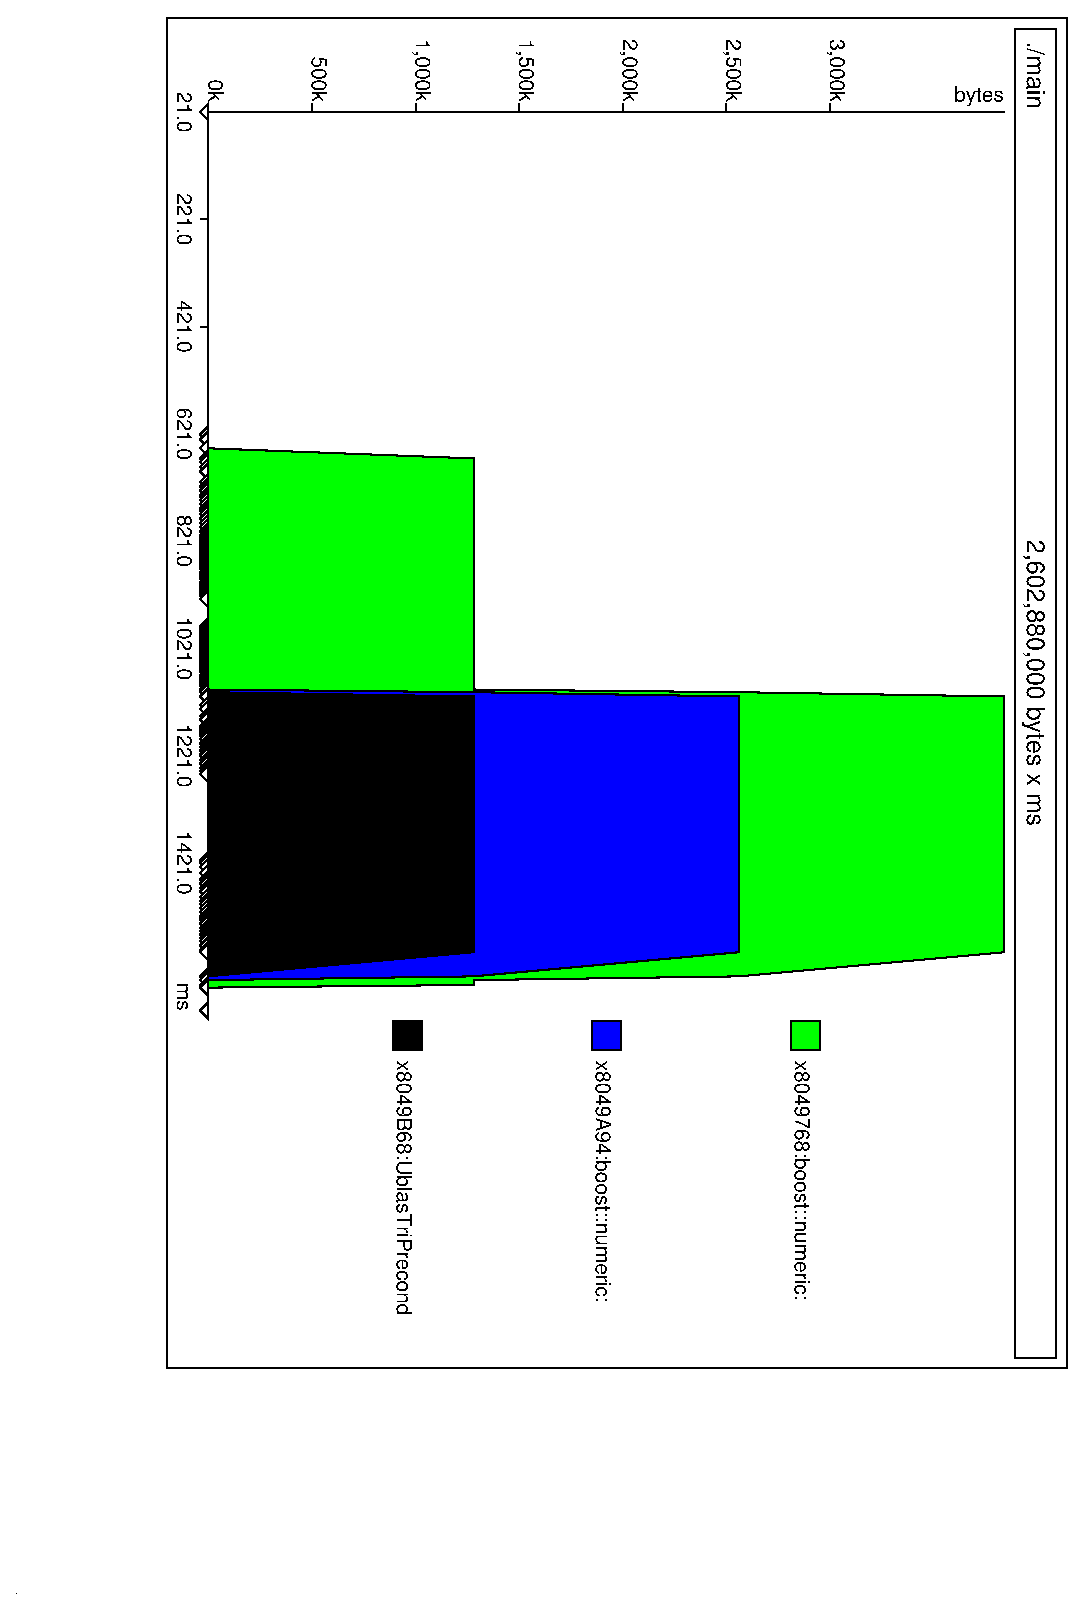
\includegraphics[height=.75\textwidth,angle=-270]{./massif.densebig.eps}
}
\subfigure[Matrice sparsa]{
\centering
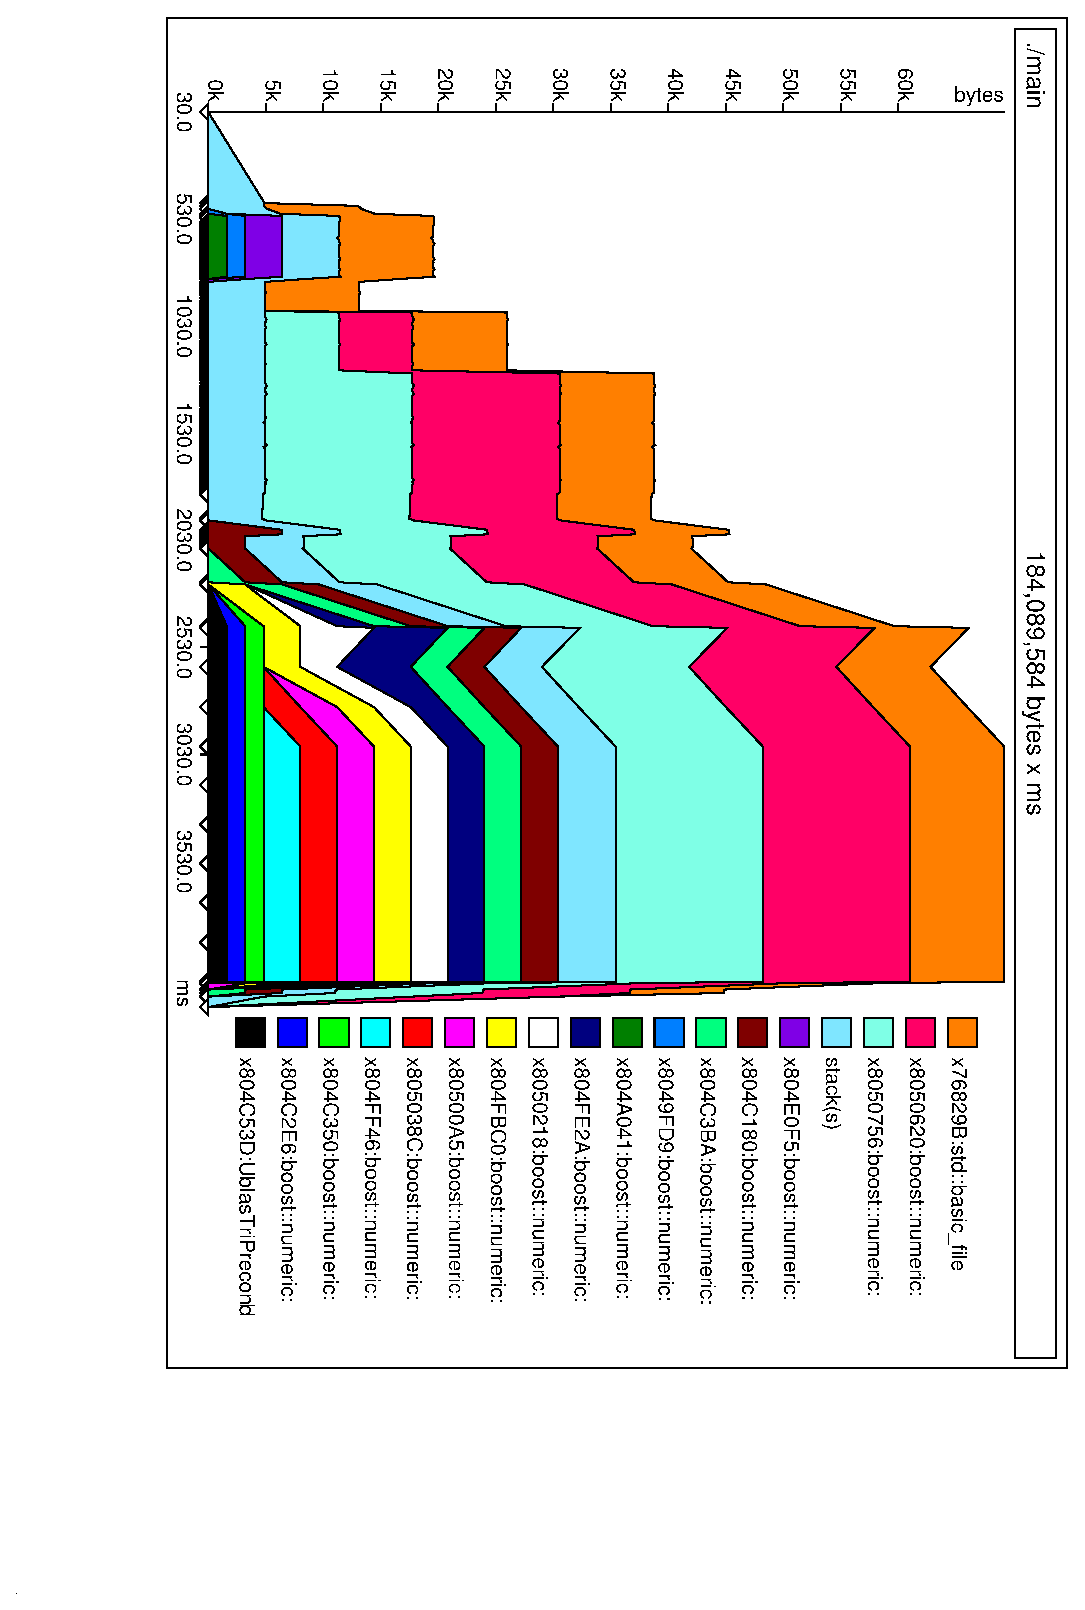
\includegraphics[height=.75\textwidth,angle=-270]{./massif.sparsebig.eps}
}
\caption{Occupazione di memoria durante l'esecuzione del programma,
  per la risoluzione di un sitema lineare quadrato di ordine 400.}
\label{fig:fin:results}
\end{figure}

I grafici generati da \texttt{valgrind} attraverso lo strumento
\texttt{massif} indicano dei valori di occupazione della memoria in
termini di \emph{spazio-tempo}: l'area sottesa alle curve misura
quanta memoria \emph{heap} \`e stata occupata, per quanto tempo. In effetti
il tempo di esecuzione del programma viene influenzato dalle
operazioni svolte da \texttt{valgrind}, quindi il dato pi\`u rilevante
\`e quello ``spaziale'' (in ordinata). In ciascun grafico si nota
quali operazioni del programma ne influenzino maggiormente le
prestazioni; confrontando i due grafici si ha un idea dell'effetto
dell'utilizzo dei due diversi formati di memorizzazione dei
dati. Informazioni dettagliate sulle misure realizzate da
\texttt{valgrind} sono riportate nel file di testo generato come
output. Per ottenere il maggior numero di indicazioni occorre
compilare il \emph{main program} con opzioni di \emph{debug}.

Si noti che, nell'implementazione proposta,
vengono utilizzati i tipi della libreria
\cpp{boost}: quando si utilizzano oggetti di tipo \cpp{matrix}, che
adottano il formato di memorizzazione pieno, l'occupazione della
memoria \`e decisamente pi\`u ingente. Il formato di memorizzazione sparso \`e adottato da
oggetti di tipo \cpp{coordinate_matrix}, grazie ai quali l'occupazione complessiva
di memoria \`e ridotta circa di un fattore 50 (nel caso di matrice
$400 \times 400$).


